\section{Kinematics}
Kinematics, often regarded as 'geometry of motion' describes motion of points (or bodies) without considering the effect of forces \cite{wikikine}. Kinematics can be separated into four steps, which are namely forward and inverse kinematics, path and trajectory planning. In this section we will first introduce the theoretical background of the aforementioned four steps then outline the implementation that arose from this theory.
\subsection{Theory}


\subsubsection{Forward Kinematics}
Forward kinematics is the problem of determination of the position and orientation of the end effector given the values for the joint variables. One common way to approach this problem is via utilizing Denavit and Hartenberg (D-H).
In D-H convention each joint is attached with one coordination frame and transformation between these frames are
expressed in four parameters \cite{wikidh}
\begin{itemize}
    \item $d$: offset along previous $z$ to the common normal
    \item $\theta$: angle about previous $z$, from old $x$ to new $x$
    \item $a$: length of the common normal. Assuming a revolute joint, this is the radius about previous $z$
    \item $\alpha$: angle about common normal, from old $z$ axis to new $z$ axis
\end{itemize}
Using the modified version of the DH-parameters results in transformation matrix between axes $n-1$ and $n$ as follows

\begin{equation}
    ^{n - 1}T_n=
    \left[\begin{smallmatrix}
              \cos\theta_n & -\sin\theta_n  & 0 & a_{n-1} \\
              \sin\theta_n \cos\alpha_{n-1} & \cos\theta_n \cos\alpha_{n-1} & -\sin\alpha_{n-1}& -d_n
              \sin\alpha_{n-1} \\
              \sin\theta_n\sin\alpha_{n-1} & \cos\theta_n \sin\alpha_{n-1} & \cos\alpha_{n-1} & d_n
              \cos\alpha_{n-1} \\
              0 & 0 & 0 & 1
    \end{smallmatrix} \right]
\end{equation}
So given all DH-parameters one can find all coordinate frames defined on the robot. These parameters can be presented
on a table, named appropriately as DH-Table, which is commonly provided by the manufacturer. In this case the table
provided by Franka documentary is tabulated in Table \ref{dhtable}. More info can be found on website of Franka Control Interface \cite{frankaweb}.

\begin{table}[ht]
    \caption{DH-parameters}
    \label{dhtable}
    \begin{center}
        \begin{tabular}{|c|c|c|c|c|}
            \hline
            \textbf{\textit{Joint}} & \textbf{\textit{a (m)}} & \textbf{\textit{d (m)}} & \textbf{\textit{ $\alpha$
                (rad)}}& \textbf{\textit{ $\theta$ (rad)}}\\
            \hline
            Joint1 & 0 & 0.333 & 0
            & $\theta_{1}$ \\
            \hline
            Joint2 & 0 & 0 & -$\pi$/2
            & $\theta_{2}$ \\
            \hline
            Joint3 & 0 & 0.316 & $\pi$/2
            & $\theta_{3}$ \\
            \hline
            Joint4 & 0.0825 & 0 & $\pi$/2
            & $\theta_{4}$ \\
            \hline
            Joint5 & -0.0825 & 0.384 & -$\pi$/2
            & $\theta_{5}$ \\
            \hline
            Joint6 & 0 & 0 & $\pi$/2
            & $\theta_{6}$ \\
            \hline
            Joint7 & 0.088 & 0 & $\pi$/2
            & $\theta_{7}$ \\
            \hline
            Flange & 0 & 0.107 & 0 & 0 \\
            \hline
        \end{tabular}
        \label{tab2}
    \end{center}
\end{table}

Utilizing this table one can calculate the end effector pose by multiplying each transformation. This equation as commonly called kinematic chain can be found below in Equation \ref{chain_eq}.

\begin{equation}
    \label{chain_eq}
    T_7^0 = T_1^0 T_2^1 T_3^2 T_4^3 T_5^4 T_6^5 T_7^6
\end{equation}

Figure \ref{robot_img} depicts the provided frames on the robot image.


\begin{figure}[ht]
    \centering
    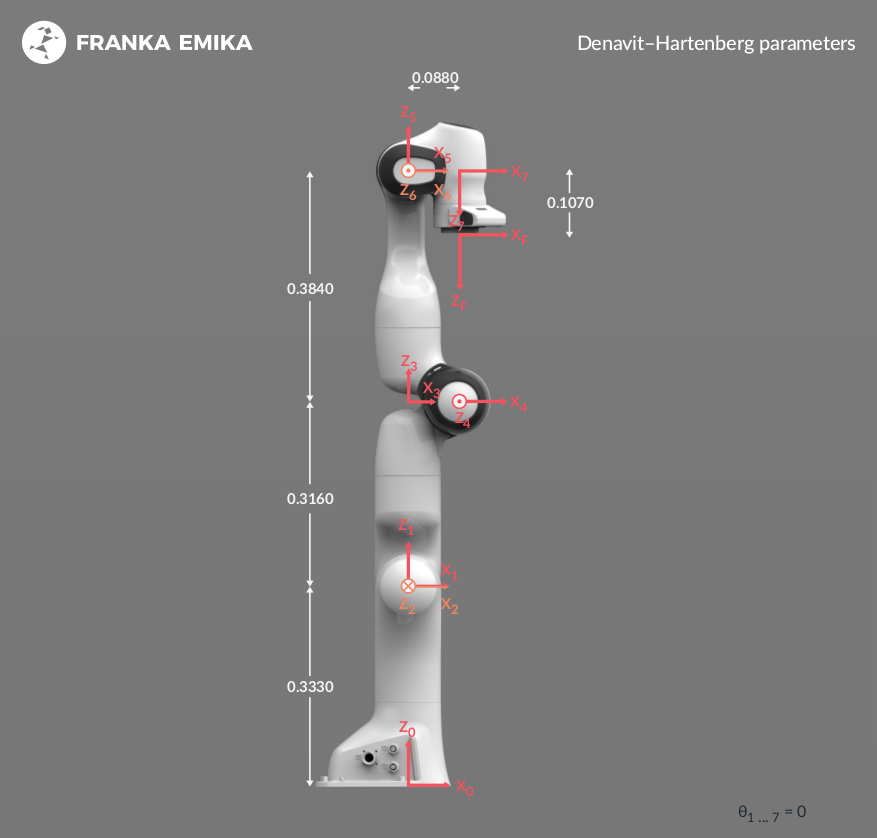
\includegraphics[width=0.45\textwidth]{images/dh-diagram.png}
    \caption{Coordinate frames on the robot}
    \label{robot_img}
\end{figure}

\subsubsection{Inverse Kinematics}
As forward kinematics determine the position and orientation of the end effector from joint variables, inverse kinematics determines the latter given the former. More generally, given a homogeneous transformation
$$
H = 
\begin{bmatrix}
R & p \\
0 & 1
\end{bmatrix}
$$
find joint variables
$$
T_n^0(q_1,...,q_n) = H
$$
Although there are closed form solutions to the system of equations, as geometry of robot gets more complex they become hard to solve analytically. In this study we used a common approach to approximate the solution of systems, namely least squares. The least-squares method finds the optimal parameter values by  minimizing the sum of squared residuals

$$S=\sum_{i=1}^{n}r_i^2.$$
\subsubsection{Path Planning}
Path planning aims to find a continuous map $g$ from start point, $g(0)$ to goal point $g(1)$ in configuration space, taking into account where the known world $W$ is occupied by obstacles or with the robot itself. With the inverse kinematics we can map these points to their corresponding configurations, namely $q_s$ and $q_g$.

In this study we don't consider obstacles, so motion planning simplifies to trajectory generation, which is enough to 'move' the robot from its former pose into the goal position with a simple check on joint limits.
\subsubsection{Trajectory Generation}
 A trajectory is a function of time $q(t)$ such that $q(t_0)=q_s$ and $q(t_f)=q_g$ (see Trajectory Planning section in \cite{spong}). Trajectory planning expands the path into a 'step-by-step plan' with the introduction of time as a variable, which than could be fed to the controller. Here 'step-by-step' posits the implicit dependency on control frequency, which in case of Panda robot is 1000Hz.
 
 Polynomials of degree n, is a common selection for parametrization of trajectories, where n is dependent on the number of constraints \cite{spong}.Having continuous position, velocity and acceleration (thus no impulsive jerk) for both initial and final configurations lays 6 constraints, so a fifth order polynomial
$$ q(t) = a_0 + a_1t + a_2t^2 + a_3t^3 + a_4t^4 + a_5t^5 $$
would suffice. Taking its derivatives one could reach at:
$$ v(t) = \Dot{q}(t) = a_1 +2 a_2t +3 a_3t^2 +4 a_4t^3 +5 a_5t^4 $$
$$ \alpha(t) = \Ddot{q}(t) = 2 a_2 + 6 a_3t + 12 a_4t^2 + 20 a_5t^3 $$
Plugging $t_0$ and $t_f$ in to above equations and then arranging them in matrix form:
$$\begin{bmatrix}
1 & t_0 & t_0^2 & t_0^3 & t_0^4 & t_0^5 \\
0 & 1 & 2t_0 & 3t_0^2 & 4t_0^3 & 5t_0^4\\
0 & 0 & 2 & 6t_0 & 12t_0^2 & 20t_0^3\\
1 & t_f & t_f^2 & t_f^3 & t_f^4 & t_f^5\\
0 & 1 & 2t_f & 3t_f^2 & 4t_f^3 & 5t_f^4\\
0 & 0 & 2 & 6t_f & 12t_f^2 & 20t_f^3\\ 
\end{bmatrix}
\begin{bmatrix}a_0\\a_1\\a_2\\a_3\\a_4\\a_5\\\end{bmatrix}
=
\begin{bmatrix}q_0\\v_0\\\alpha_0\\q_f\\v_f\\\alpha_f\end{bmatrix}$$
Solving this linear system of equations would result in coefficients $a_i$ that can be used to parametrize the trajectory in the appropriate profiles. These profiles can be seen on Figure \ref{quintics}

 \begin{figure}[ht]
  \centering
  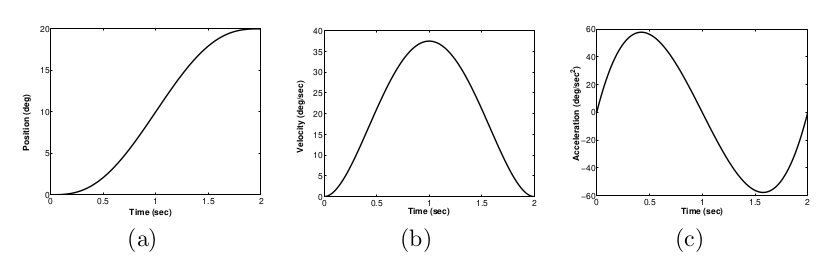
\includegraphics[width=0.45\textwidth]{images/quintics.png}
  \caption{(a) Quintic Polynomial Trajectory. (b) Velocity Profile  (c) Acceleration Profile (figure obtained from \cite{spong}])}
  \label{quintics}
 \end{figure}


% Tell how we used changed frankaros
\subsection{Implementation}
When divided into two main packages the runtime process simplifies to following steps:
\begin{itemize}
    \item Kinematics: Scans the target provides requested image and pose pairs to the vision package
    \item Vision: Processes aforementioned inputs to provide 3-float vector corresponding the position of the target point, accompanied by information on the possible approach orientation for insertion.
    \item Kinematics: Inserts the needle in to the target point, while keeping the needle on a straight line when inside the phantom.
\end{itemize}

The interaction between these two packages can be illustrated with the Figure \ref{overview}.

\begin{figure}
    \label{overview}
    \caption{Overview of the package interaction}
    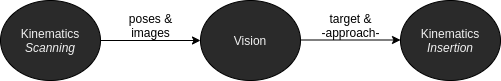
\includegraphics[width=0.5\textwidth]{images/overview}
\end{figure}


To utilize ROS and already existing Franka ROS Library the kinematics package is formed by the following nodes:
\begin{itemize}
    \item simple\_scanner: Employs the scanning routine around the target point to generate image and pose pairs necessary for vision. Holds SphericalScanner class.
    \item simple\_capture: Communicates with scanner node to save necessary information at every stop. Holds ImageCapture class.
    \item simple\_inserter: Manages the insertion procedure given a target point and a peak point. Holds Inserter class.
    \item simple\_planner: Trajectory planner node, plans and publishes the plans on desired control frequency given the goal pose in homogenous transformation. Holds TrajectoryPlanner class.
    \item simple\_goal: A goal definer for debugging purposes. It is created to test the kinematics application not depending on the state of the vision package. Holds GoalSetter class.
\end{itemize}
These active nodes are utilizing the following modules
\begin{itemize}
    \item simple\_node: Holds the Communicative\_Node parent class which is inherited by most of the classes in this package. It maps all the necessary topics while keeping track of whether the process is on simulation. It also has some commonly used methods by most of the other modules such as waiting for execution or getting joint states.
    \item simple\_robot: Holds Robot class that is imported whenever forward kinematics is needed to be employed. It uses the inherent links that are provided by manufacturer and also necessary end effectors which all are broadcasted via tf package from ROS.
    \item simple\_ik: Holds Inverse\_Kinematics class which is executed whenever there is need of inverse kinematics calculation.
    \item simple\_quintics: Includes mostly static mathematical methods that are necessary to plan a trajectory with quintic polynomials.
    \item simple\_cartographer: Helps the trajectory planner when it needs to make end effector point at some point during scanning or insertion processes.
\end{itemize}

A diagram to help visualize the kinematics package can be found in Appendix, Figure \ref{app_overview}.

The entire process can be summarized as
\begin{itemize}
    \item Scanner node starts a spherical scan pattern around the approximate target point whilst directing the camera towards it with the help of Cartographer. During which there is a checkerboard for calibration purposes.
    \item Capture node captures images and poses to pass on Vision package.
    \item Receiving the target point and approach direction Inserter class first peaks at the target point where it can insert the needle on a straight line, then inserts it to the target.
\end{itemize}
During this process Cartographer helps directing the end effector to the desired orientation, Robot class tracks the provided and developped coordinate frames and joint limits, inverse kinematics  calculates the joint states that are needed to be reached for the target point at each step. All of which are passed to the planner which outputs a plan quantized with the control frequency, or in case of insertion fed directly to the command topic of robot.


The entire implementation of this package is done on most recent versions of both Python and ROS, which during the time of the study were 3.9 and Noetic respectively.
Indeed the provided robot framework runs on the Python 2.7 and ROS Kinetic, which has potential to pose a problem via incompatibility.
Although at the end flexible ROS architecture allowed us to run the package on another computer on the same network and communicate controller via topics.
One more implementation note is the use of a modified fork of franka\_ros package.
To be able to communicate the current execution state, franka\_ros package is modified accordingly and stored in a separate fork from the original clone that was provided.
